\chapter{Dataset and Methodology}\label{ch:method}

\section{Dataset}

We use the Malayalam split of Naamapadam~\cite{mhaske2023naamapadam}
(\texttt{ai4bharat/naamapadam}). Each example is a tokenized sentence with
one IOB2 tag per word. Because of limited compute (a single RTX-class GPU),
we train on the first 50{,}000 of the 716{,}652 training sentences
(Table~\ref{tab:splits}).

\begin{table}[H]
\centering
\caption{Dataset splits used.}
\label{tab:splits}
\begin{tabular}{lrrrrr}
\toprule
Split & Sentences & Tokens & PER & ORG & LOC \\
\midrule
Train (subset) & 50{,}000 & 456{,}631 & 35{,}057 & 16{,}265 & 21{,}333 \\
Validation     & 3{,}618  & 33{,}371  & 2{,}569  & 1{,}182  & 1{,}610 \\
Test           & 965$^\ast$ & 8{,}534 & 714      & 309      & 482 \\
\bottomrule
\multicolumn{6}{l}{\footnotesize $^\ast$9 of the 974 rows are empty or malformed and are discarded.}
\end{tabular}
\end{table}

The data is heavily imbalanced (Figure~\ref{fig:tagdist}). The \texttt{O}
tag covers 74.1\% of tokens, and \texttt{I-LOC} only 0.9\%, because most
Malayalam place names are a single agglutinated word.

\begin{figure}[H]
\centering
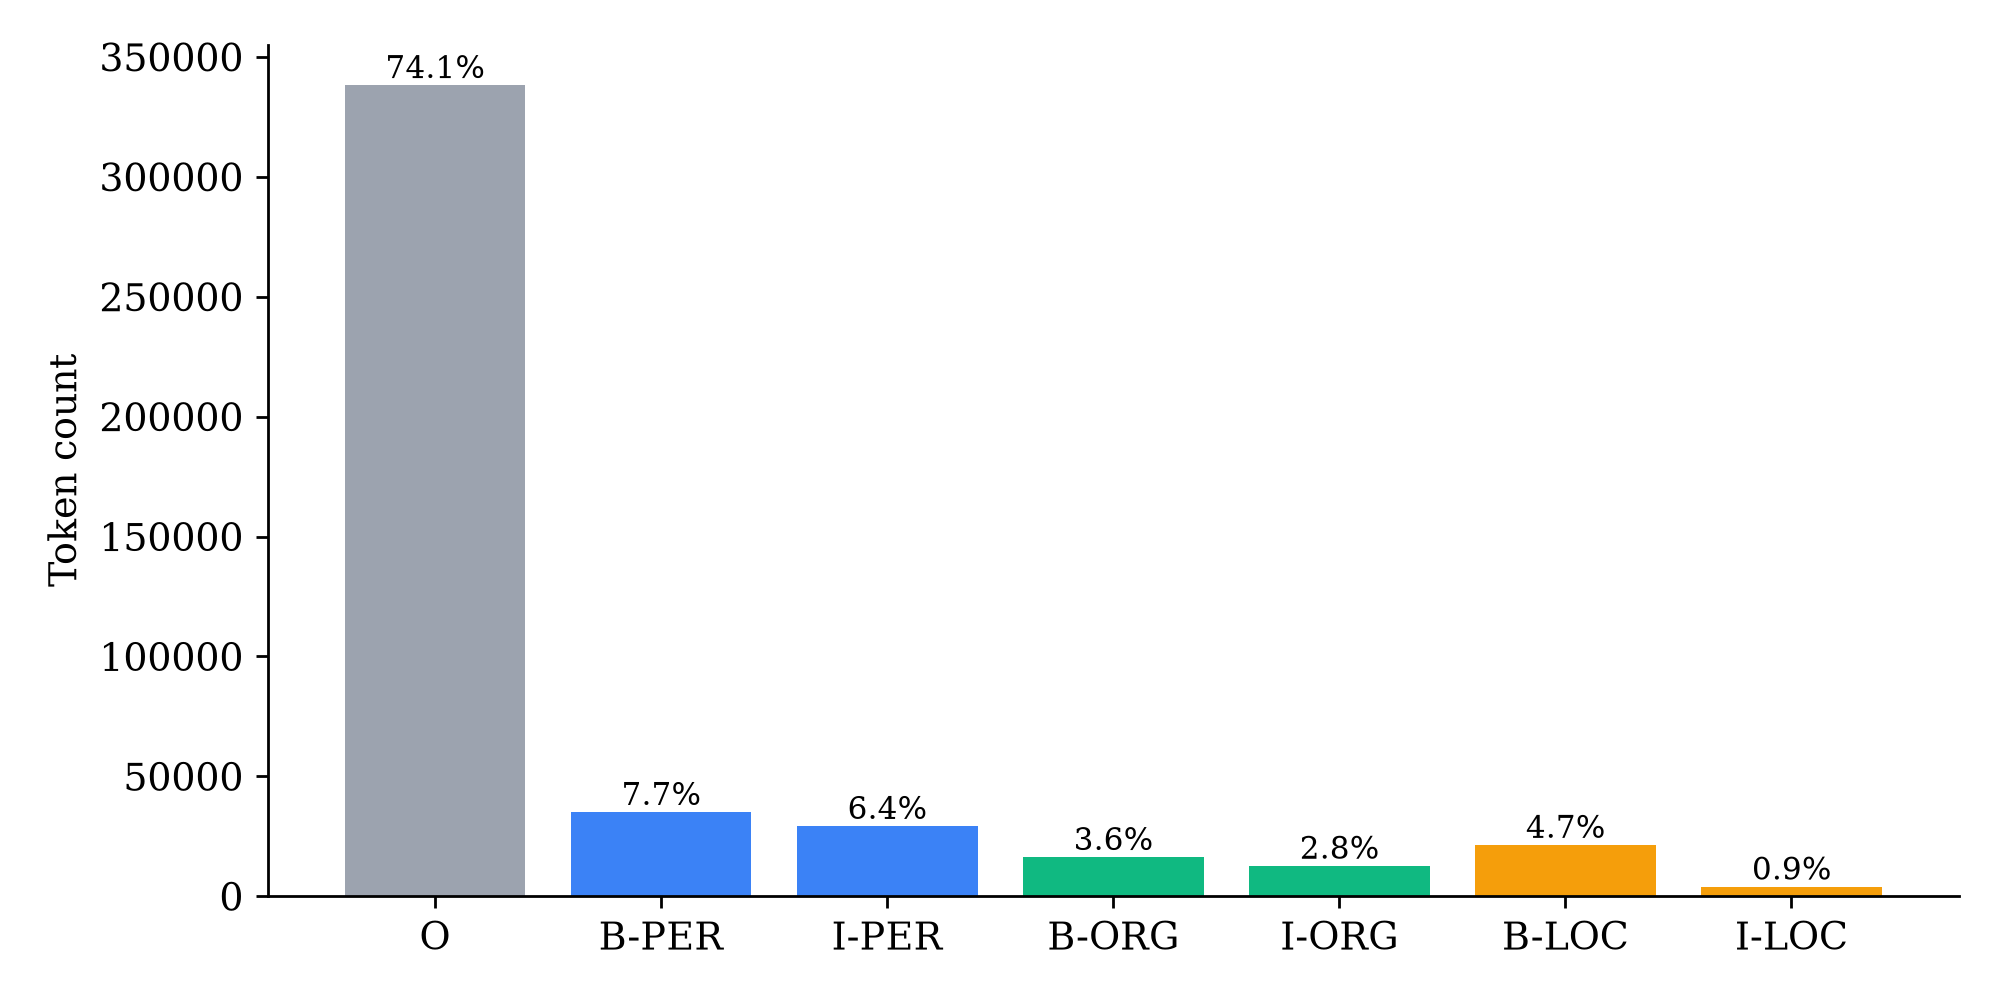
\includegraphics[width=0.72\textwidth]{tag_distribution.png}
\caption{Tag distribution in the training subset.}
\label{fig:tagdist}
\end{figure}

\section{Subword Label Alignment}

The IndicBERTv2 tokenizer splits words into subword pieces, on average
\textbf{1.56 subwords per word} on the test set, so words and labels no
longer line up one to one. Using the tokenizer's \texttt{word\_ids()}
mapping~\cite{wolf2020transformers}, the \emph{first} subword of each word
receives the word's label. Continuation subwords and special tokens receive
$-100$, which the loss ignores. Inputs are truncated or padded to 128
subwords.

\begin{example}
\emph{(Pinarayi, Vijayan, samsarichu)} with tags (\texttt{B-PER},
\texttt{I-PER}, \texttt{O}) tokenized as
\texttt{[CLS] pina \#\#rayi vijayan sam \#\#sari \#\#chu [SEP]} gets labels
$(-100, \texttt{B-PER}, -100, \texttt{I-PER}, \texttt{O}, -100, -100, -100)$.
\end{example}

\section{Model Architecture}

\begin{figure}[H]
\centering
\resizebox{\textwidth}{!}{%
\begin{tikzpicture}[
  node distance=0.5cm,
  box/.style={draw, rounded corners, align=center, minimum height=1.1cm, text width=2.3cm, font=\small},
  arr/.style={-{Stealth[length=2.5mm]}, thick}]
\node[box, fill=gray!10] (in) {Malayalam\\sentence};
\node[box, fill=yellow!15, right=of in] (tok) {WordPiece\\tokenizer};
\node[box, fill=blue!12, right=of tok, text width=2.6cm] (enc) {IndicBERTv2\\(12 layers, 768-d)};
\node[box, fill=blue!5, right=of enc] (lin) {Dropout +\\Linear $768{\rightarrow}7$};
\node[box, fill=green!12, right=of lin] (crf) {CRF (Viterbi)\\or softmax};
\node[box, fill=orange!15, right=of crf] (out) {IOB2 tags\\+ rule overlay};
\draw[arr] (in) -- (tok);
\draw[arr] (tok) -- (enc);
\draw[arr] (enc) -- node[above, font=\scriptsize]{$\mathbf{h}_i$} (lin);
\draw[arr] (lin) -- node[above, font=\scriptsize]{$\mathbf{e}_i$} (crf);
\draw[arr] (crf) -- (out);
\end{tikzpicture}}
\caption{System architecture.}
\label{fig:arch}
\end{figure}

\textbf{Encoder.} \texttt{ai4bharat/IndicBERTv2-MLM-only}~\cite{doddapaneni2023towards}
is a 12-layer BERT-base Transformer (about 278M parameters). Bidirectional
self-attention lets the representation $\mathbf{h}_i$ of a stem subword use
both its own case suffix and the surrounding words. The backbone can be
switched to MuRIL or mBERT in \texttt{config.py}.

\textbf{Emissions.} A dropout layer and a linear layer produce tag scores
$\mathbf{e}_i = W\,\mathrm{Dropout}(\mathbf{h}_i) + \mathbf{b} \in \mathbb{R}^{7}$.

\subsection{Baseline: Softmax with Class Weights}

As in the base paper, each position is classified independently,
$\hat{y}_i = \arg\max_c e_{i,c}$. To counter the imbalance, the
cross-entropy loss uses inverse-frequency weights normalised by their
maximum, $w_c \propto N / (K\, n_c)$, where $n_c$ is the count of tag $c$:
\begin{equation}\label{eq:wce}
\mathcal{L}_{\mathrm{WCE}} = -\frac{\sum_{i} w_{y_i} \log \mathrm{softmax}(\mathbf{e}_i)_{y_i}}{\sum_{i} w_{y_i}}.
\end{equation}

\subsection{Proposed: Conditional Random Field}

A linear-chain CRF~\cite{lafferty2001conditional, lample2016neural} learns a
transition matrix $A \in \mathbb{R}^{7 \times 7}$ and scores a whole tag
sequence:
\begin{equation}
s(\mathbf{x}, \mathbf{y}) = \sum_{i} e_{i, y_i} + \sum_{i>1} A_{y_{i-1}, y_i}, \qquad
p(\mathbf{y} \mid \mathbf{x}) = \frac{\exp s(\mathbf{x}, \mathbf{y})}{\sum_{\mathbf{y}'} \exp s(\mathbf{x}, \mathbf{y}')}.
\end{equation}
Training minimises $-\log p(\mathbf{y}^{\ast} \mid \mathbf{x})$ using the
forward algorithm, and decoding uses Viterbi. Both run in $O(mK^2)$ time.
Because $A$ is learned, transitions that never occur in training, such as
\texttt{O}$\rightarrow$\texttt{I-ORG}, are strongly penalised, so the
decoder prefers consistent multi-word spans. The CRF loss is \emph{not}
class-weighted.

\section{Training Setup}

\begin{table}[H]
\centering
\caption{Training configuration (identical for both models).}
\label{tab:hparams}
\begin{tabular}{ll}
\toprule
Optimiser & AdamW~\cite{loshchilov2019decoupled}, lr $3\times10^{-5}$, weight decay 0.01 \\
Schedule & 10\% linear warm-up, then cosine decay \\
Batch / epochs / max length & 32 / 3 / 128 subwords \\
Precision & FP16 mixed precision~\cite{micikevicius2018mixed} \\
Model selection & Best validation entity-level F1 \\
\bottomrule
\end{tabular}
\end{table}

\section{Rule Overlay at Inference}

Naamapadam annotates only PER, ORG and LOC. For the demo, words the model
tags as \texttt{O} are checked against simple rules. Malayalam month names
and date formats such as DD-MM-YYYY are tagged DATE. Tokens containing
Arabic or Malayalam digits, optionally followed by unit words such as
\emph{shathamanam} (percent) or \emph{kodi} (crore), are tagged CARDINAL.
These rules are not used in any reported metric.
